\newcommand{\antOffx}{-0.4}
\newcommand{\antOffy}{ 0.3}

% Triangle:
\newcommand{\origin }{0.0}
\newcommand{\baseOffx }{6.5}
% (setq baseOffx '6.5)
% (setq tg '4.0)
% (* tg (sin (- (/ pi 2) (asin (/ tg baseOffx))))) 3.153
% (* tg (cos (- (/ pi 2) (asin (/ tg baseOffx))))) 2.461
\newcommand{\sinTheta }{3.153}
\newcommand{\cosTheta }{2.461}

% Parallel lines:
% (* (sqrt (- (* baseOffx baseOffx) (* tg tg))) (cos (asin (/ tg baseOffx)))) 4.038
\newcommand{\parrOff }{4.038}

\newcommand{\triThick }{1.1mm}    % Triangle line thickness
\newcommand{\linThick }{0.3mm}    % Line thickness

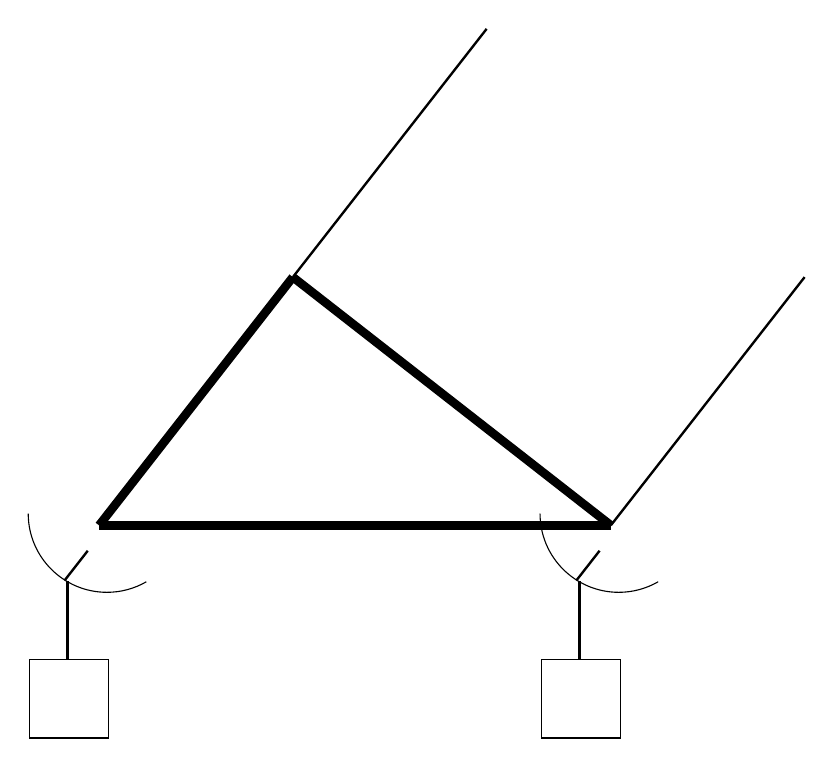
\begin{tikzpicture}

  % Parallel lines:
  \draw[line width= \linThick, black] (\cosTheta *2,           \sinTheta *2) -- (\cosTheta ,            \sinTheta );
  \draw[line width= \linThick, black] (\cosTheta *2+\parrOff , \sinTheta   ) -- (\cosTheta + \parrOff , \origin   );

  % Triangle:
  \draw[line width= \triThick, black] (\baseOffx , \origin   ) -- (\cosTheta , \sinTheta );
  \draw[line width= \triThick, black] (\cosTheta , \sinTheta ) -- (\origin   , \origin   );
  \draw[line width= \triThick, black] (\baseOffx , \origin   ) -- (\origin   , \origin   );

  % Telescopes:
    % Dish:
    \draw (\origin   -0.5+\antOffx, \origin -0.15+\antOffy ) arc (180:300:1cm);
    \draw (\baseOffx -0.5+\antOffx, \origin -0.15+\antOffy ) arc (180:300:1cm);
    % Neck:
    \draw[line width= \linThick, black] (\baseOffx +\antOffx , -2.0+\antOffy ) -- (\baseOffx +\antOffx , -1.0+\antOffy );
    \draw[line width= \linThick, black] (\origin   +\antOffx , -2.0+\antOffy ) -- (\origin   +\antOffx , -1.0+\antOffy );
    % Feed:
    \draw[line width= \linThick, black] (\antOffx+\cosTheta*1.12-2.5,            \sinTheta*1.12-\sinTheta-1+\antOffy) -- (\antOffx +\cosTheta -2.5,            \sinTheta -\sinTheta -1+\antOffy );
    \draw[line width= \linThick, black] (\antOffx+\cosTheta*1.12-2.5+\baseOffx , \sinTheta*1.12-\sinTheta-1+\antOffy) -- (\antOffx +\cosTheta -2.5+\baseOffx , \sinTheta -\sinTheta -1+\antOffy );

  % Pedestal:
  \draw [black] (-2.5+1.62,            -2.7) rectangle (-1.5+1.62,            -1.7);
  \draw [black] (-2.5+1.62+\baseOffx , -2.7) rectangle (-1.5+1.62+\baseOffx , -1.7);

\end{tikzpicture}

%%% Local Variables:
%%% mode: latex
%%% TeX-master: "../Lecture"
%%% End: